\section{Iteration 9: Decomposition of the Health Monitoring Unit}
\label{add:it9}

\subsection{Step 1: Identify candidate drivers}
\label{add:it9/drivers}

\npar Two quality attributes were assigned to the health monitoring unit:

\begin{itemize}
  	\item Av1': Measurement database failure.
  	\begin{itemize}
  	  \item The failure is detected in less then five seconds.
  	\end{itemize}
  	\item Av2': Missing measurements.
  	\begin{itemize}
  	  \item Failure of an internal component should be detected within one
  	  minute.
  	\end{itemize}
\end{itemize}

\subsection{Step 2: Choose design concepts}
\label{add:it9/concepts}

\subsubsection{Tactics}
\label{add:it9/tactics}

\npar Since only the detection part of the availability attributes was assigned
to the health monitoring unit, the tactics used in this iteration will be based
upon that assumption. In section \ref{add:it1} we discussed the best detection
tactic and this resulted in the usage of a heartbeat. The usage of heartbeat
will be the (only) tactic in this iteration.

\subsubsection{Design Patterns}
\label{add:it9/patterns}

\npar There was no design pattern found to support the notification
functionality in combination with the heartbeat tactic.

\subsection{Step 3: Instantiate architectural elements and allocate responsibilities}
\label{add:it9/elements}

\begin{figure}[H]
	\begin{centering}
		% TODO Figure
		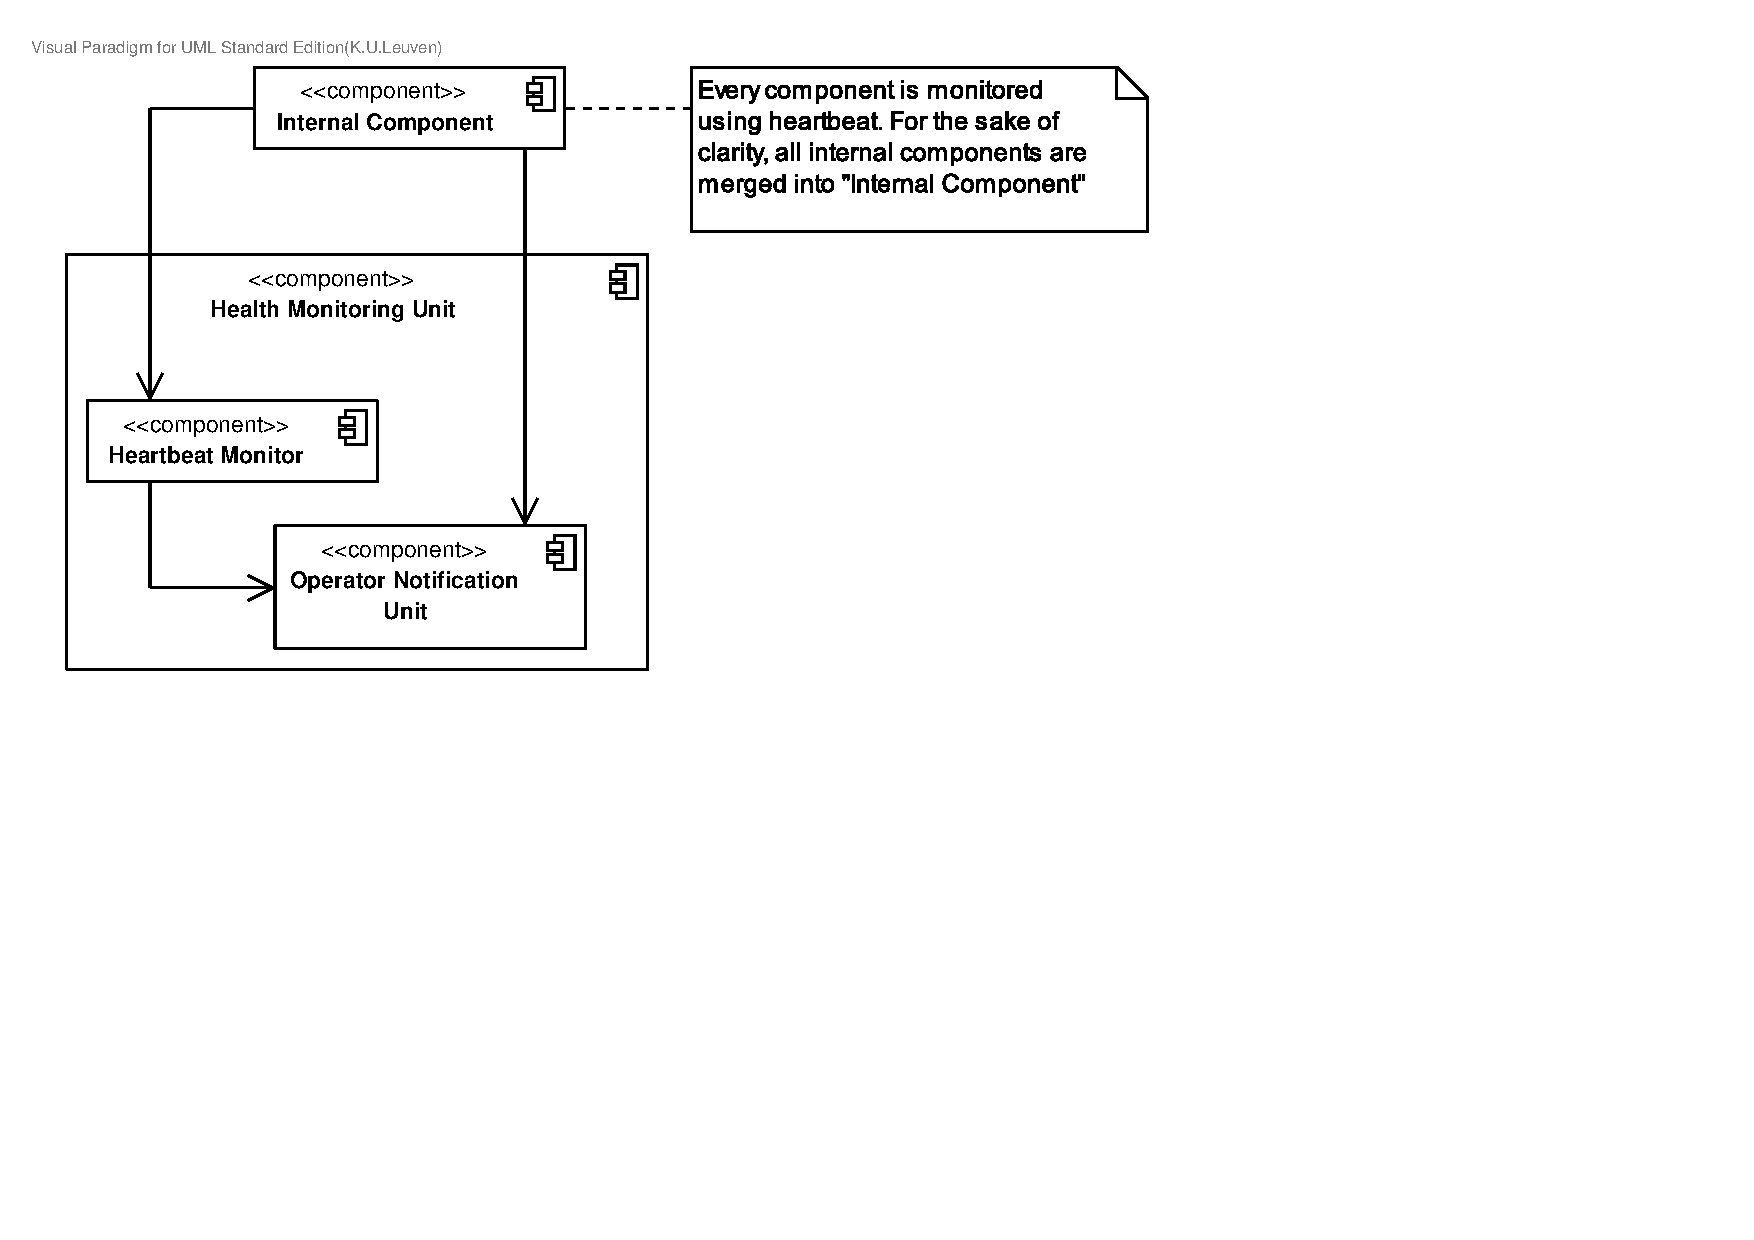
\includegraphics[width=\textwidth]{figs/add-it9-elements.pdf}
		\caption{Overview of the instantiated child elements in the Health Monitoring
		Unit}
		\label{fig:it9/elements}
	\end{centering}
\end{figure}

\npar The design is relatively simple. There are only two components, they are
together with all their associations depicted in figure
%TODO: gaat er geen commentaar komen op het feit dat ons notification gedrag
% over 2 plaatsen verspreid is ?
\subsubsection{Operator Notification Unit}

\npar This unit is purely responsible for the notification of ReMeS operators. A
notification request can enter this unit either from the heartbeat monitor or
from an external component.

\subsubsection{Heartbeat Monitor}

\npar The heartbeat monitor is a registering point for other components to
confirm that they are still up and running. When a component does not give a
heartbeat signal, it is assumed that that component is crashed and approriate
action is undertaken (i.e. a ReMeS operator is notified).

\subsection{Step 4: Define interfaces for instantiated elements}
\label{add:it9/interfaces}

\subsubsection{Operator Notification Unit}

\paragraph{OperatorNotificationAPI}
%TODO: moet er uberhaupt een message zijn of is dit altijd gewoon hetzelfde
% message (namelijk een crash) ?
\npar This interface offers a \method{notify(Message)} method. The
purpose of this method is notifying a ReMeS operator with the given message
parameter. 

\subsubsection{Heartbeat Monitor}

\paragraph{HealthMonitorAPI}
%TODO: parameter van de pulse methode
\npar Since there is a need for other component to give a signal that they are
still alive a method \method{pulse()} is included. This is the only method this
interface offers.

\begin{figure}[H]
	\begin{centering}
		% TODO Figure
		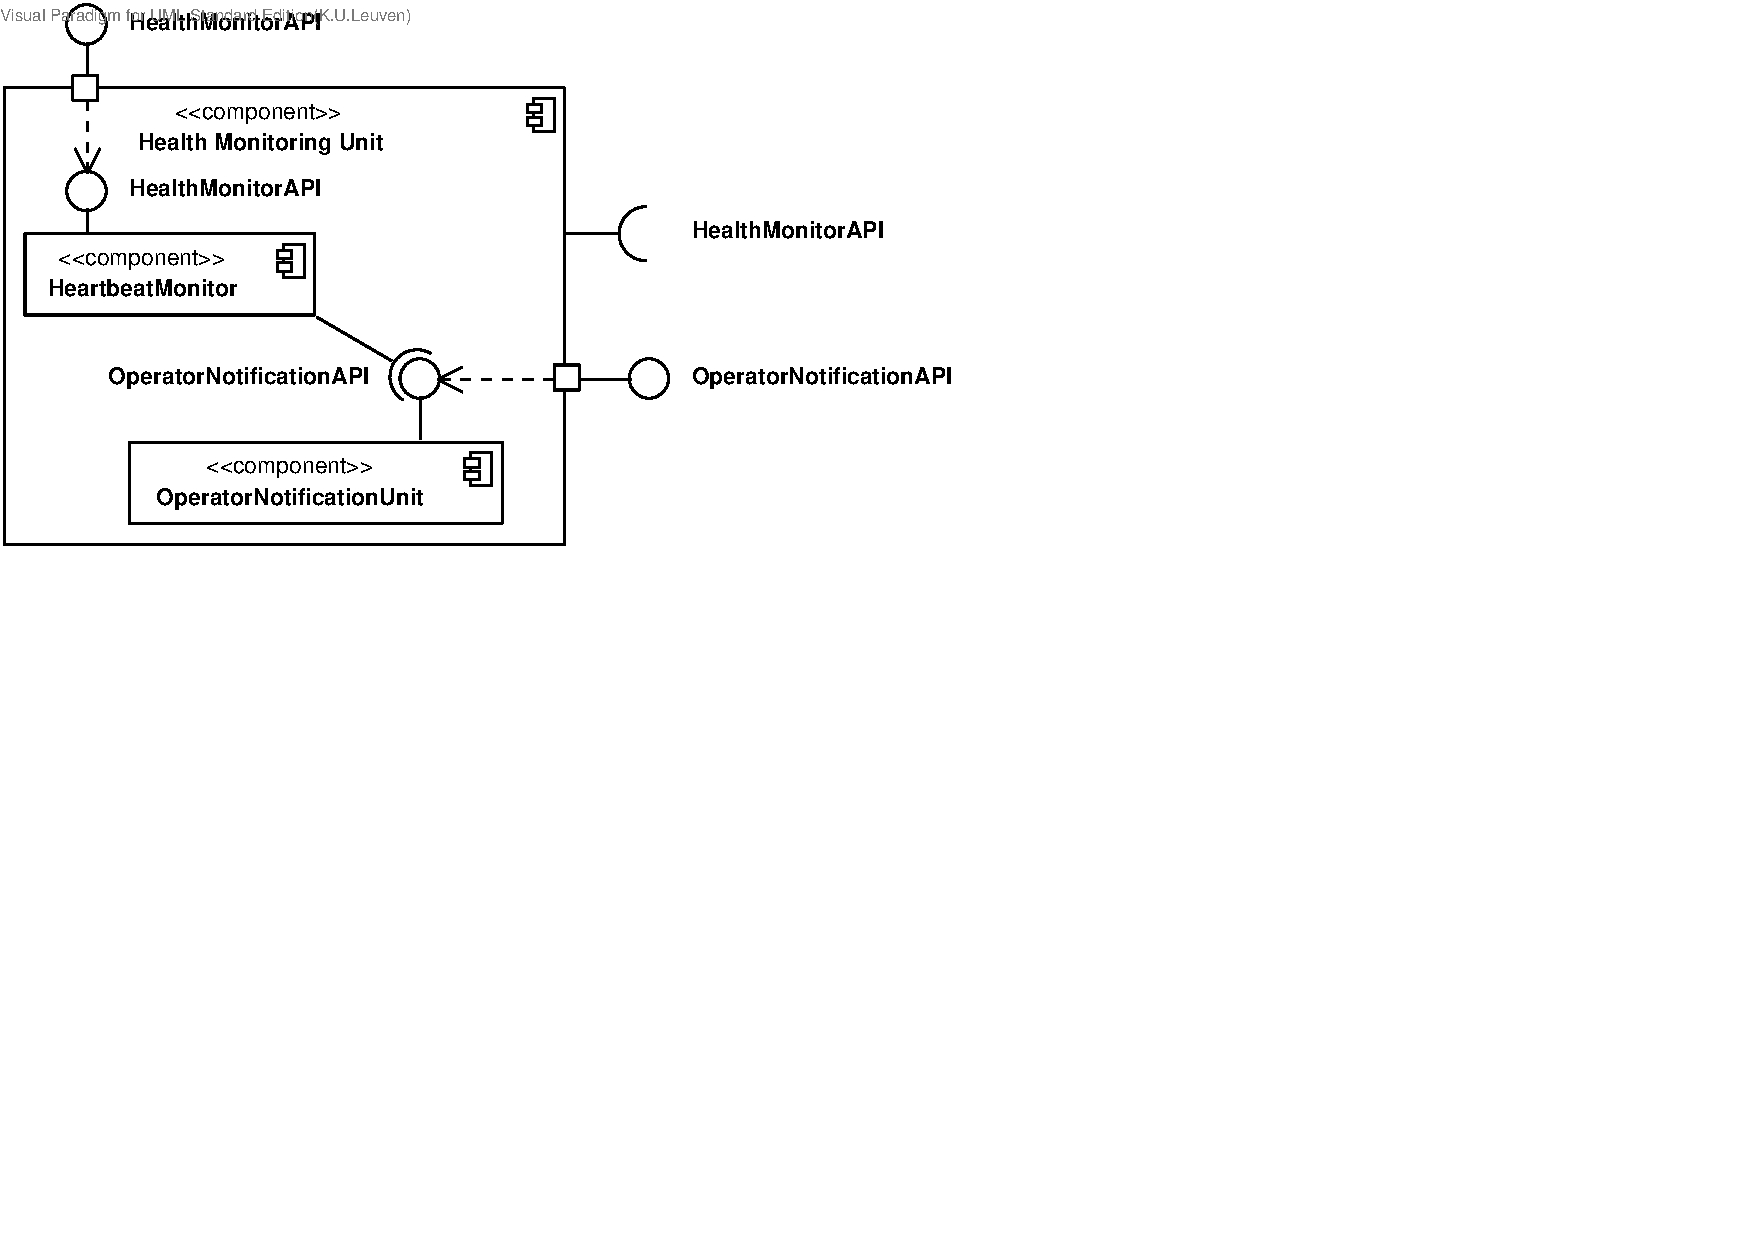
\includegraphics[width=\textwidth]{figs/add-it9-interfaces.pdf}
		\caption{Overview of the interfaces and components in the Health Monitoring
		Unit}
		\label{fig:it9/interfaces}
	\end{centering}
\end{figure}

\subsection{Step 5: Verify and refine}
\label{add:it9/verification}

\npar The assigned parts of Av1' and Av2' were resolved in this iteration
through the use of the Heartbeat Monitor and the Operator Notification Unit.
